This documentation describes the software: \textit{PyETL} \& \textit{DecubiTection}, a software transforming CSV data into an OMOP common data model and using machine learning to identify potential decubitus risks, regarding hospital patients.

The software is divided into three main systems: \textit{ETL process}, \textit{Machine Learning / Decubitus risk prediction} and \textit{Front-end}. 
Each system is able to run on its own and only depends on the results of the preceding subsystem stored in a database.

\begin{figure}[htbp]
\centerline{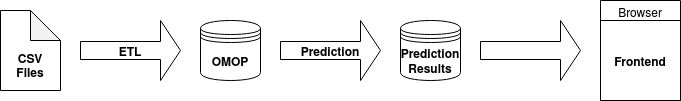
\includegraphics[width=1\linewidth]{images/DecubitusPipeline.png}}
\caption{Overview over the subsystems and their relations}
\label{fig:pipeline}
\end{figure}

There is the possibility to schedule the ETL-Process and the decubitus 
detection algorithm in a certain interval through a cron job. 
For this purpose, a Python script is provided which is able to create a cron job with the required parameters such as database host, password, etc.

\subsection{ETL process}
The purpose of the ETL-Process is to map medical data, provided by a set of CSV files formatted according to the specifications of §21 Paragraphs 4 and 5 KHEntgG, into the OMOP common data model (CDM).
This step is required, since the later described machine learning system learns and predicts, using data, gathered from an OMOP CDM. 

The ETL-Process requires certain preconditions. The CSV files are required to only contain valid and new data. Otherwise, the ETL-Process might fail or inconsistent data will be inserted into the OMOP database. 

The following explanation describes the ETL-Process for a single patient. 
In the first step, data from the \textit{FALL.csv} file gets extracted and will be inserted in the OMOP database, according to table \ref{etl-person}.
Since the provided data does not contain information about the patient's race and ethnicity, default values will be inserted. 
In case the patient's location is not already stored in the database, the ETL-Process will supplement this information, as depicted in table \ref{etl-location}.
If in two or more visits, the information differs, only the most up-to-date information will be inserted.
For every row in the FALL.csv file, a new visit will be inserted into VISIT\_OCCURRENCE as shown in table \ref{etl-visit}.
If the care site, the patient is currently located in, is not stored in the CARE\_SITE table, a new record is added, as illustrated in table \ref{etl-caresite}.

In the next step, all values - concerning the patient - from the \textit{LABOR.csv} file will be inserted, as depicted in table \ref{etl-labor}.
As the file only contains measurements, rows containing a different domain ID than "Measurement" will be skipped. 
If that happens, a warning will be printed onto STDERR. 
Similarly, the ETL-Process maps the data from \textit{MEASUREMENT.csv} to the database, as illustrated in table \ref{etl-measurement}.

The data from the \textit{ICD.csv} file is mapped as follows. If the domain ID of a row is an "Observation", a new observation will be inserted into OBSERVATION. 
If the value of "sekundaer\_kode" is empty, only one data record will be added as depicted in table \ref{etl-icd-observation}, in which case "ICD.icd\_kode" is mapped to observation\_source\_value.
If "sekundaer\_kode" is not empty, a second record will be added, where "ICD.sekundaer\_kode" is mapped to observation\_source\_value.

If the domain ID is a "Condition", instead of an "Observation", a new condition will be inserted in the database, as depicted by table \ref{etl-icd-condition}.
Similar to the previously described case, if a "sekundaer\_kode" is available, another record will be added. This is illustrated in table \ref{etl-icd-condition}. 
Additionally, if "lokalisation" is not empty, a new record will be inserted in the database, as shown in table \ref{etl-icd-location}.
The same applies if "diagnosesicherheit" is not empty, in which case the data is mapped as depicted in table \ref{etl-icd-diagnosensicherheit}.
Both records will be connected to the previously generated records through a fact relationship in both directions, as illustrated in table \ref{fact-relation}. 
If the domain id is neither "Condition" nor "Observation", the row will be skipped and a warning will be printed.

From \textit{OPS.csv}, the ETL-Process maps all procedures - concerning the patient - to the database, as illustrated in table \ref{etl-ops}.
Equally as described earlier, if a row contains a domain id, different from "Procedure", the row will be skipped and a warning will be printed.

%FALL.csv
\begin{table} [htbp]
\begin{tabular}{|l|l|}
 \hline
  \textbf{source column} & \textbf{destination column} \\
  \hline
  FALL.patienten\_nummer & PERSON.person\_id \\
  FALL.last\_record & PERSON.gender\_concept\_id \\
  FALL.geburtsjahr & PERSON.year\_of\_birth \\
  FALL.geburtsmonat & PERSON.month\_of\_birth \\
  "Unknown" & PERSON.race\_concept\_id \\
  "Not Hispanic" & PERSON.ethnicity\_concept\_id \\
  FALL.gender\_source\_value & PERSON.geschlecht \\
  \textit{LOCATION}.location\_id & PERSON.location \\
  \hline
\end{tabular}
\caption{Insert data from FALL.csv into table PERSON.}
\label{etl-person}
\end{table}

% LOCATION
\begin{table} [htbp]
\begin{tabular}{|l|l|}
  \hline
  \textbf{source column} & \textbf{destination column} \\
  \hline
  FALL.city & LOCATION.city \\
  FALL.zip & LOCATION.zip \\
  \hline
\end{tabular}
\caption{Insert a patient's location from FALL.csv to LOCATION.}
\label{etl-location}
\end{table}

\begin{table} [htbp]
\begin{tabular}{|l|l|}
  \hline
  \textbf{source column} & \textbf{destination column} \\
  \hline
  FAB.FAB & CARE\_SITE.care\_site\_name \\
  \hline
\end{tabular}
\caption{Insert a patient's visits to VISIT\_OCCURRENCE.}
\label{etl-visit}
\end{table}

% VISIT OCCURRENCE
\begin{table} [htbp]
\begin{tabular}{|l|l|}
  \hline
  \textbf{source column} & \textbf{destination column} \\
  \hline
  FALL.kh\_internes\_kennzeichen & VISIT\_OCCURRENCE.visit\_occurrence\_id \\
  FALL.aufnahmeanlass & VISIT\_OCCURRENCE.visit\_concept\_id \\
  FALL.aufnahmedatum & VISIT\_OCCURRENCE.visit\_start\_date \\
  FALL.entlassungsdatum & VISIT\_OCCURRENCE.visit\_end\_date \\
  "Visit derived from EHR record" & VISIT\_OCCURRENCE.visit\_type\_concept\_id \\
  FALL.aufnahmeanlass & VISIT\_OCCURRENCE.visit\_source\_value \\
  FALL.aufnahmegrund & VISIT\_OCCURRENCE.admitting\_source\_value \\
  FALL.entlassungsgrund & VISIT\_OCCURRENCE.discharge\_to\_source\_value \\
  \textit{CARE\_SITE}.care\_site\_id & VISIT\_OCCURRENCE.care\_site\_name \\
  \hline
\end{tabular}
\caption{Insert a new care site.}
\label{etl-caresite}
\end{table}

% LABOR -> MEASUREMENT
\begin{table} [htbp]
\begin{tabular}{|l|l|}
  \hline
  \textbf{source column} & \textbf{destination column} \\
  \hline
  LABOR.concept\_id & MEASUREMENT.measurement\_concept\_id \\
  LABOR.timestamp & MEASUREMENT.measurement\_date \\
  LABOR.timestamp & MEASUREMENT.measurement\_datetime \\
  "Lab Result" & MEASUREMENT.measurement\_type\_concept\_id \\
  LABOR.value & MEASUREMENT.value\_as\_number \\
  LABOR.concept\_id & MEASUREMENT.measurement\_source\_concept\_id \\
  LABOR.LOINC & MEASUREMENT.measurement\_source\_value \\
  LABOR.unit & MEASUREMENT.unit\_source\_value \\
  \hline
\end{tabular}
\caption{Insert measurement from LABOR.csv into MEASUREMENT.}
\label{etl-labor}
\end{table}

% MESSUNGEN -> MEASUREMENT
\begin{table} [htbp]
\begin{tabular}{|l|l|}
  \hline
  \textbf{source column} & \textbf{destination column} \\
  \hline
  MESSUNGEN.concept\_id & MEASUREMENT.measurement\_concept\_id \\
  MESSUNGEN.timestamp & MEASUREMENT.measurement\_date \\
  MESSUNGEN.timestamp & MEASUREMENT.measurement\_datetime \\
  "From physical examination" & MEASUREMENT.measurement\_type\_concept\_id \\
  MESSUNGEN.concept\_id & MEASUREMENT.measurement\_source\_concept\_id \\
  MESSUNGEN.LOINC & MEASUREMENT.measurement\_source\_value \\
  MESSUNGEN.value & MEASUREMENT.value\_as\_number \\
  MESSUNGEN.unit & MEASUREMENT.unit\_source\_value \\
  \hline
\end{tabular}
\caption{Insert measurement from MEASUREMENT.csv into MEASUREMENT.}
\label{etl-measurement}
\end{table}

%ICD.csv
\begin{table} [htbp]
\begin{tabular}{|l|l|}
  \hline
  \textbf{source column} & \textbf{destination column} \\
  \hline
  ICD.concept\_id & OBSERVATION.observation\_concept\_id \\
  FALL.aufnahmedatum & OBSERVATION.observation\_date \\
  "Observation recorded from EHR" & OBSERVATION.observation\_type\_concept\_id \\
  ICD.concept\_id & OBSERVATION.observation\_source\_concept\_id \\
  ICD.icd\_kode / ICD.sekundaer\_kode & OBSERVATION.observation\_source\_value \\
  \hline
\end{tabular}
\caption{Insert observation from ICD.csv into the OBSERVATION.}
\label{etl-icd-observation}
\end{table}

% LOCALISATION
\begin{table} [htbp]
\begin{tabular}{|l|l|}
  \hline
  \textbf{source column} & \textbf{destination column} \\
  \hline
  ICD.lokalisation & OBSERVATION.observation\_concept\_id \\
  FALL.aufnahmedatum & OBSERVATION.observation\_date \\
  "Observation recorded from EHR" & OBSERVATION.observation\_type\_concept\_id \\
  ICD.lokalisation & OBSERVATION.observation\_source\_value \\
  ICD.lokalisation & OBSERVATION.value\_as\_string \\
  \hline
\end{tabular}
\caption{Insert information about the location from 
    ICD.csv to OBSERVATION.}
\label{etl-icd-location}
\end{table}

% FACT RELATIONSHIP
\begin{table} [htbp]
\begin{tabular}{|l|l|}
  \hline
  \textbf{source column} & \textbf{destination column} \\
  \hline
  \textless table1\textgreater & FACT\_RELATIONSHIP.domain\_concept\_id\_1 \\
  \textit{\textless table1\textgreater}.observation\_id & FACT\_RELATIONSHIP.fact\_id\_1 \\
  \textless table2\textgreater & FACT\_RELATIONSHIP.domain\_concept\_id\_2 \\
  \textit{\textless table2\textgreater}.observation\_id & FACT\_RELATIONSHIP.fact\_id\_2 \\
  "Finding associated with/Associated with finding" & FACT\_RELATIONSHIP.relationship\_concept\_id \\
  \hline
\end{tabular}
\caption{Connect two entries through a fact relation.}
\label{fact-relation}
\end{table}

% diagnosensicherheit
\begin{table} [htbp]
\begin{tabular}{|l|l|}
  \hline
  \textbf{source column} & \textbf{destination column} \\
  \hline
  ICD.diagnosensicherheit & OBSERVATION.observation\_concept\_id \\
  FALL.aufnahmedatum & OBSERVATION.observation\_date \\
  "Observation recorded from EHR" & OBSERVATION.observation\_type\_concept\_id \\
  ICD.diagnosensicherheit & OBSERVATION.observation\_source\_value \\
  ICD.diagnosensicherheit & OBSERVATION.value\_as\_string \\
  \hline
\end{tabular}
\caption{Insert information about the diagnostic reliability from 
    ICD.csv to OBSERVATION.}
\label{etl-icd-diagnosensicherheit}
\end{table}

% CONDITION OCCURRENCE
\begin{table} [htbp]
\begin{tabular}{|l|l|}
  \hline
  \textbf{source column} & \textbf{destination column} \\
  \hline
  ICD.concept\_id & CONDITION\_OCCURRENCE.condition\_concept\_id \\
  FALL.aufnahmedatum & CONDITION\_OCCURRENCE.condition\_start\_date \\
  FALL.aufnahmedatum & CONDITION\_OCCURRENCE.condition\_start\_datetime \\
  ICD.diagnoseart & CONDITION\_OCCURRENCE.condition\_type\_concept\_id \\
  ICD.concept\_id & CONDITION\_OCCURRENCE.source\_concept\_id \\
  ICD.icd\_kode/ICD.sekundaer\_kode & CONDITION\_OCCURRENCE.source\_value \\
  \hline
\end{tabular}
\caption{Insert conditions from ICD.csv to CONDITION\_OCCURRENCE.}
\label{etl-icd-condition}
\end{table}

% OPS.csv
\begin{table} [htbp]
\begin{tabular}{|l|l|}
  \hline
  \textbf{source column} & \textbf{destination column} \\
  \hline
  OPS.concept\_id & PROCEDURE\_OCCURRENCE.procedure\_occurrence\_id \\
  OPS.ops\_datum & PROCEDURE\_OCCURRENCE.procedure\_date \\
  OPS.ops\_datum & PROCEDURE\_OCCURRENCE.procedure\_datetime \\
  "Procedure recorded as diagnostic code" & PROCEDURE\_OCCURRENCE.procedure\_type\_concept\_id \\
  OPS.ops\_kode & PROCEDURE\_OCCURRENCE.procedure\_source\_value \\
  OPS.concept\_id & PROCEDURE\_OCCURRENCE.procedure\_source\_concept\_id \\
  \hline
\end{tabular}
\caption{Insert procedures from OPS.csv into PROCEDURE\_OCCURRENCE.}
\label{etl-ops}
\end{table}

\newpage
\subsection{Decubitus Risk Prediction}
The decubitus risk prediction is provided by a neural network, trained on patient data of the OMOP CDM. 
The network takes a number of clinical findings as input and predicts binary the risk of the patient developing a pressure ulcer in the near future.
The specific findings used as input are determined by selecting the unique concept ids from the database which describe the patient's condition at the time a pressure ulcer is diagnosed.
Therefore only findings are selected that could possibly be connected to the risk of developing a decubitus.

In the training process, old patient data is sampled at different moments pairing the information on the patient's condition given at this point and the binary label whether a pressure ulcer will be diagnosed within the next n dates contained in the database.
N is a number to be configured prior to the training.
The sampled data is split into a testset and a trainset.
The network is trained only on the trainset, therefore the testset contains new unseen samples on which the network can be evaluated.

Once a neural network is trained on the trainset, validated on the testset and the classification threshold is selected, it can be loaded into the actual prediction pipeline.
The Pipeline takes the latest patient data from the OMOP CDM as input and calculates the decubitus risk prediction. 
Afterwards, using gradient backpropagation, the Pipeline determines the importance of the different inputs to the calculated prediction.
The most important clinical findings are filtered to reject meaningless Information and the top ten remaining facts are stored together with the prediction, to be displayed in the front-end.

\subsection{Front-End}

The front-end is a web application, running on a dedicated server, reachable only from the network of the medical institution. 
The patient data is protected by a login page, requiring a valid username and password. 
The data is extracted from the database, where the results of the decubitus risk detection pipeline are stored. 
The patient data is illustrated inside a table, where patients, potentially developing a decubitus are marked in red. 
The results can be downloaded and printed as a PDF file. 
Necessary parameters e.g. database connection settings can be configured as command line parameters on startup of the application. 